\documentclass[12pt, letterpaper]{article}
\usepackage{listings}
\usepackage{xcolor}
\usepackage{amssymb}
\usepackage{amsmath}
\usepackage{graphicx}
\usepackage{hyperref}
\usepackage{url}
\usepackage{float}
\usepackage{tikz}

\emergencystretch=3em
\Urlmuskip=0mu plus 1mu

% --- Style pendukung ilustrasi TikZ Neural Network ---
\definecolor{mygreen}{RGB}{0,140,80}
\definecolor{myblue}{RGB}{0,90,160}
\definecolor{myred}{RGB}{180,0,0}

\tikzset{
    nnnode/.style={circle, draw, minimum size=0.8cm, inner sep=0pt},
    nnconnect/.style={-, thick, gray},
}

% --- Konfigurasi Warna dan Style ---
\definecolor{codegreen}{rgb}{0,0.6,0}
\definecolor{codegray}{rgb}{0.5,0.5,0.5}
\definecolor{codepurple}{rgb}{0.58,0,0.82}
\definecolor{backcolour}{rgb}{0.95,0.95,0.92}

\lstdefinestyle{mystyle}{
    backgroundcolor=\color{backcolour},
    commentstyle=\color{codegreen},
    keywordstyle=\color{magenta},
    numberstyle=\tiny\color{codegray},
    stringstyle=\color{codepurple},
    basicstyle=\ttfamily\footnotesize,
    breakatwhitespace=false,
    breaklines=true,
    captionpos=b,
    keepspaces=true,
    numbers=left,
    numbersep=5pt,
    showspaces=false,
    showstringspaces=false,
    showtabs=false,
    tabsize=2,
    language=Python
}

\lstset{style=mystyle}

\title{Bagaimana CNN (\textit{Convolutional Neural Network)} bekerja?}
\author{Fajar Adie Santosa (\href{https://www.instagram.com/debug_stack/}{@debug.stack})}
\date{2026}

\begin{document}
\maketitle

\newpage
\tableofcontents
\newpage


\section*{Pendahuluan}
\addcontentsline{toc}{section}{Pendahuluan}
(TAMBAHKAN PRE-REQUISITE UNTUK BISA MEMAHAMI DOKUMEN INI : KALKULUS, ALJABAR LINEAR)
Model CNN (\textit{Convolutional Neural Network}) adalah salah satu jenis jaringan saraf tiruan yang digunakan untuk pengolahan data seperti gambar atau time series. Di era sekarang ini, membuat model CNN hanya memerlukan import library seperti TensorFlow atau PyTorch dan menulis beberapa baris kode untuk membangun model CNN. Namun, pernahkah berpikir, bagaimana sebenarnya CNN bekerja?mengapa memerlukan parameter dari library ini? dari rasa penasaran tersebut, dilakukan pembuatan ulang CNN dari awal menggunakan Python dan NumPy, tanpa menggunakan library deep learning apapun. Dengan begitu, dapat memahami bagaimana CNN bekerja. 
% \begin{enumerate}
%     \item input data berupa gambar, pada projek ini kita akan menggunakan dataset MNIST, yang berisi gambar digit 0-9.(done)
%     \item melakukan proses konvolusi pada gambar input dan menambahkan bobot dan bias, kemudian hasilnya akan diteruskan ke aktivasi ReLU (pada projek ini kita menggunakan ReLU, karena ReLU lebih cepat dan lebih baik untuk mengatasi masalah vanishing gradient) (done)
%     \item melakukan proses pooling (done)
%     \item melakukan proses pengulangan
%     \item melakukan proses flattening(done), yaitu mengubah data 2D menjadi 1D
%     \item melakukan proses fully connected layer, yaitu menghubungkan semua neuron pada layer sebelumnya ke neuron pada layer berikutnya(done)
%     \item melakukan proses softmax, yaitu mengubah output menjadi probabilitas (done)
%     \item melakukan proses backpropagation, yaitu menghitung gradien dan memperbarui bobot dan bias
%     \item melakukan proses evaluasi model
% \end{enumerate}

\section*{STEP 1: Input}
\addcontentsline{toc}{section}{STEP 1: Input}
Pada projek ini, input yang digunakan adalah gambar, menggunakan dataset MNIST (yang didapat dari \href{https://www.kaggle.com/datasets/hojjatk/mnist-dataset}{kaggle}). Terus, bagaimana Neural Network (NN) bisa memahami gambar? sepahaman saya, gambar merupakan kumpulan dari pixel, dan pixel merupakan kumpulan dari angka. Namun, angka dari gambar itu mempresentasikan apa? angka dari gambar itu mempresentasikan intensitas cahaya, dimana semakin besar angka, semakin terang pixel tersebut. Untuk lebih jelasnya, kalian bisa mempelajarinya di \href{https://www.youtube.com/watch?v=pj9-rr1wDhM}{youtube ini}. Menurut saya, penjelasan di youtube ini sangat mudah dipahami dan ada visual yang membantu untuk memahami konsep CNN ini.

\begin{figure} [H]
  \centering
  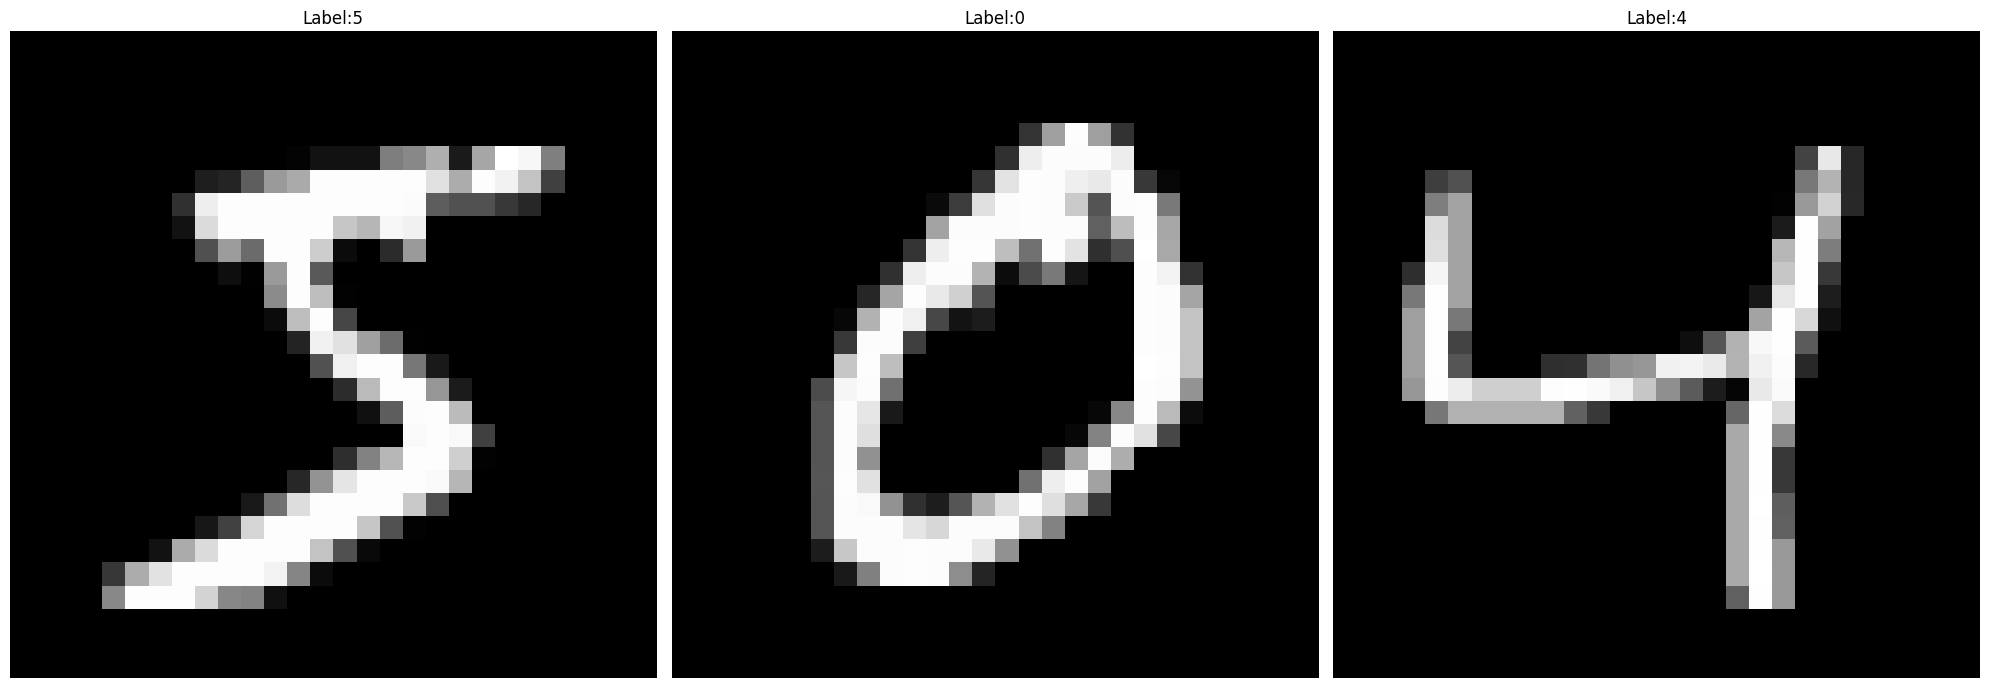
\includegraphics[width=0.5\textwidth]{mnist-example.png}
  \caption{Contoh gambar digit dari dataset MNIST}
  \label{fig:perceptron}
\end{figure}

Karena dataset didapat dari Yann LeCun, maka diperlukan library idx2numpy untuk mengubah dataset menjadi numpy array.
\begin{lstlisting}[language=Python, caption=Contoh kode untuk mengubah dataset menjadi numpy array]
import idx2numpy
# for training
x_train=idx2numpy.convert_from_file("/kaggle/input/datasets/hojjatk/mnist-dataset/train-images.idx3-ubyte")
y_train=idx2numpy.convert_from_file("/kaggle/input/datasets/hojjatk/mnist-dataset/train-labels.idx1-ubyte")

# for test
x_test=idx2numpy.convert_from_file("/kaggle/input/datasets/hojjatk/mnist-dataset/t10k-images.idx3-ubyte")
y_test=idx2numpy.convert_from_file("/kaggle/input/datasets/hojjatk/mnist-dataset/t10k-labels.idx1-ubyte")

\end{lstlisting}
intinya tambahkan juga untuk normalisasi data, karena data gambar memiliki nilai pixel 0-255, sehingga perlu dinormalisasi menjadi 0-1. Normalisasi ini dilakukan dengan membagi nilai pixel dengan 255.0. Dengan begitu, model CNN dapat lebih cepat dan lebih baik dalam belajar dari data gambar. Dengan rumus min-max normalisasi, yaitu:
\begin{equation}
    x_{norm} = \frac{x}{255.0}, x \in [0, 1]
\end{equation}
karena sangat mempengaruhi proses training.

\section*{STEP 2: Convolution dan ReLU}
\addcontentsline{toc}{section}{STEP 2: Convolution dan ReLU}
\subsection*{Convolution}
\addcontentsline{toc}{subsection}{Convolution}
Sebelum kita membahas lebih dalam tentang convolution, kita perlu memahami arti kernel. 
Kernel merupakan filter atau matriks kecil yang digunakan untuk mendeteksi fitur. Kernel ini akan melakukan proses konvolusi pada gambar input, dimana kernel akan menggeser posisi pada gambar input dan melakukan perkalian elemen demi elemen antara kernel dan bagian dari gambar input yang sedang diproses. 

\begin{figure} [H]
  \centering
  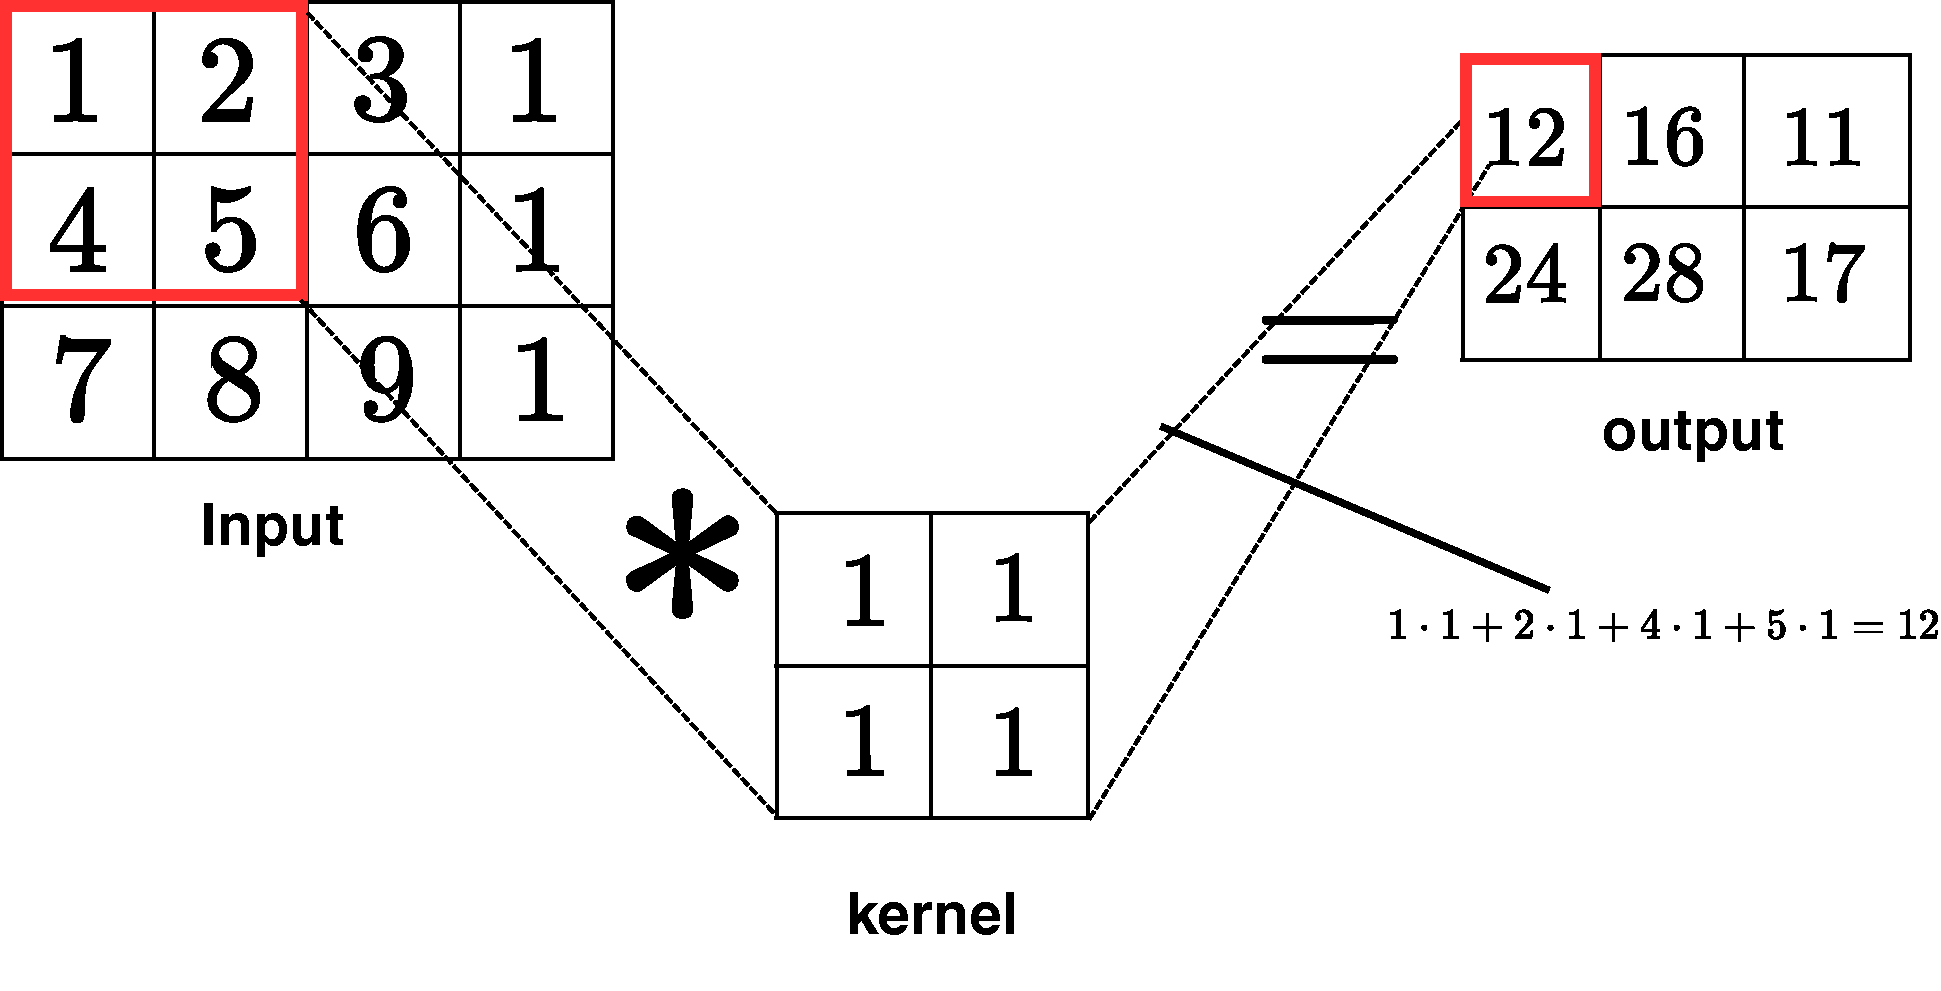
\includegraphics[width=0.5\textwidth]{operator.pdf}
  \caption{Ilustrasi proses konvolusi pada gambar input dengan kernel}
  \label{fig:konvolusi-operator}
\end{figure}

Dari kernel yang bisa digeser posisinya, itu ada nama nya, yaitu stride. Stride merupakan berapa langkah pergeseran kernel pada gambar input. Semakin besar stride, semakin cepat proses konvolusi. Untuk rumus ukuran output dari proses konvolusi:\\
\begin{equation}
H_{\text{out}} = \frac{(H + 2 * \text{pad} - K_{h})}{S} + 1
\end{equation}
yang dimana, $K$ adalah panjang kernel, $H$ adalah tinggi input (jumlah baris gambar/feature map).
\begin{equation}
W_{\text{out}} = \frac{(W_{\text{input}} + 2 * \text{pad} - K_{w})}{S} + 1
\end{equation}
Kemudian, kita lanjut arti konvolusi. Konvolusi merupakan proses perkalian elemen demi elemen antara kernel dan bagian dari gambar input, kemudian hasil perkalian tersebut dijumlahkan dan ditambahkan bias, sehingga menghasilkan output. Output dari proses konvolusi ini disebut feature map. Untuk ilustrasi proses konvolusi bisa dilihat pada gambar \ref{fig:konvolusi-operator}.

\subsection*{ReLU}
\addcontentsline{toc}{subsection}{ReLU}
ReLU (\textit{Rectified Linear Unit}) merupakan fungsi aktivasi yang digunakan untuk mengubah nilai negatif menjadi nol, dan nilai positif tetap.
\begin{figure} [H]
  \centering
  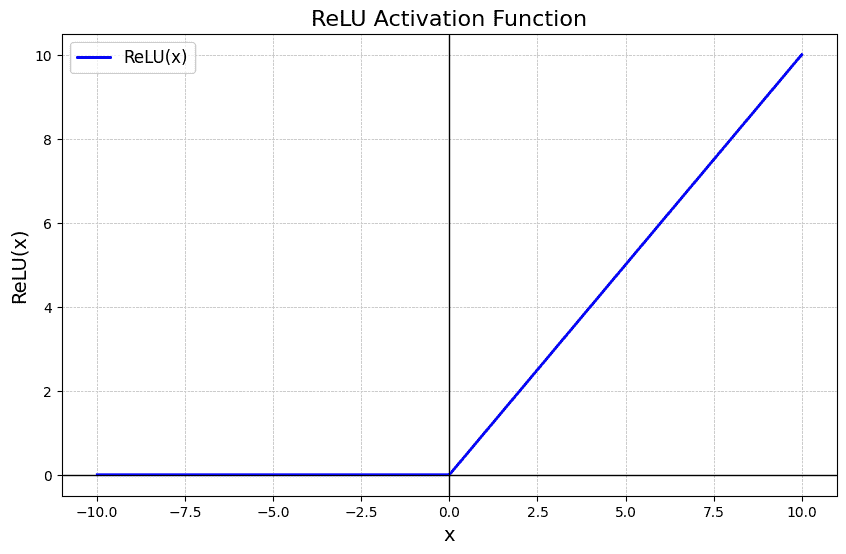
\includegraphics[width=0.5\textwidth]{Relu-activation-function.png}
  \caption{Relu Activation (\href{https://www.geeksforgeeks.org/deep-learning/relu-activation-function-in-deep-learning/}{sumber:geeksforgeeks})}
  \label{fig:relu-activation}
\end{figure}
Pada projek ini kita menggunakan ReLU sebagai fungsi aktivasi, karena berdasarkan penelitian (cari penelitiannya), ReLU lebih cocok untuk menyelesaikan masalah konvolusi. Aktivasi fungsi ReLU ini akan diterapkan pada hidden layer neural network.

\subsection*{Image-to-Column(im2col)}
\addcontentsline{toc}{subsection}{Image-to-Column}
Kalau konvolusi diimplementasikan dengan for-loop biasa (geser kernel piksel demi piksel), prosesnya akan sangat lambat di Python/NumPy, karena NumPy dioptimasi untuk operasi matriks berukuran besar (perkalian matriks/vektorisasi), bukan untuk loop bertingkat. Trik yang umum dipakai adalah im2col (image-to-column): setiap patch gambar yang akan dikalikan dengan kernel diubah menjadi satu baris pada matriks besar, sehingga seluruh proses konvolusi bisa dihitung sebagai satu kali perkalian matriks saja
\begin{lstlisting}[language=Python, caption=Fungsi im2col untuk mengubah patch gambar menjadi baris
matriks]
def im2col(x, kernel_size, stride=1):
    """
    Mengubah setiap patch gambar menjadi satu baris matrix.

    Input:
        x            : (N, C, H, W)
        kernel_size  : (KH, KW)
        stride       : langkah pergeseran kernel

    Output:
        cols         : (N * H_out * W_out, C * KH * KW)
    """

    N, C, H, W = x.shape

    KH, KW = kernel_size

    # Ukuran output convolution
    H_out = (H - KH) // stride + 1 # untuk menentukan ukuran kernel pada height
    W_out = (W - KW) // stride + 1 # untuk menentukan posisi  kernel pada weight

    # Tempat menyimpan semua patch
    cols = np.empty(
        (N, H_out, W_out, C, KH, KW),
        dtype=x.dtype
    )

    # Ambil setiap posisi kernel
    for i in range(KH):
        for j in range(KW):

            cols[:, :, :, :, i, j] = (
                x[
                    :,
                    :,
                    i:i + stride * H_out:stride,
                    j:j + stride * W_out:stride
                ]
                .transpose(0, 2, 3, 1)
            )

    # Ubah semua patch menjadi baris
    cols = cols.reshape(
        N * H_out * W_out,
        C * KH * KW
    )

    return cols
\end{lstlisting}

Setelah gambar diubah menjadi matriks $cols$ berukuran ($N \cdot H_{\text{out}} \cdot W_{\text{out}}, C \cdot K_{h} \cdot K_{w}, F$), dan kernel juga diratakan (reshape) menjadi matriks berukuran ($C \cdot K_{h} \cdot K_{w}, F$) dengan $F$ adalah jumlah filter, maka konvolusi cukup dihitung dengan satu kali perkalian matriks : $\text{cols} \odot W_{\text{col}}$

\subsection*{Convolution Forward}
\addcontentsline{toc}{subsection}{Conv Forward}
Dengan bantuan im2col, forward pass dari layer convolution bisa ditulis sebagai berikut: ubah input menjadi cols, kalikan dengan kernel yang sudah diratakan, tambahkan bias, lalu bentuk ulang hasilnya menjadi feature map

\begin{lstlisting}[language=Python, caption=Forward pass layer convolution]
  def conv2d_forward(x, W, b, stride=1):

    N, C, H, W_input = x.shape
    F, _, KH, KW = W.shape

    # Padding
    x_pad = x

    # Ambil semua patch
    cols = im2col(
        x_pad,
        kernel_size=(KH, KW),
        stride=stride
    )

    # Ubah kernel menjadi matrix
    W_col = W.reshape(F, -1).T

    # Matrix multiplication
    Z = cols @ W_col + b
    
    pad=0
    
    # Kembalikan ke bentuk feature map
    H_out = (H + 2 * pad - KH) // stride + 1
    W_out = (W_input + 2 *pad - KW) // stride + 1

    Z = Z.reshape(
        N,
        H_out,
        W_out,
        F
    )

    Z = Z.transpose(0, 3, 1, 2) # (N, H_out, W_out, F) transpose(0,3,1,2) ->  (N, F, H_out, W_out)

    conv_cache = (
        x_pad,
        W,
        stride,
        cols,
        x.shape
    )

    return Z, conv_cache

def maxpool_forward(x, size=2, stride=2):
    """
    x : input gambar
    
    Max pooling forward. Nilai yang diambil hanya nilai yang terbesar dari kernel
    """
    n, c, h, width = x.shape

    h_out = (h - size) // stride + 1 # karena channel yang dipakai hanya 1, berarti 1.1 = 1
    w_out = (width - size) // stride + 1

    out = np.empty((n, c, h_out, w_out), dtype=x.dtype)

    for i in range(h_out):
        for j in range(w_out):
            h_start = i * stride
            w_start = j * stride

            window = x[
                :,
                :,
                h_start:h_start + size,
                w_start:w_start + size
            ] # window ini hanya yang dimodif height dan weight + size...

            out[:, :, i, j] = window.max(axis=(2, 3)) # :, : -> 1. Input Image, 2. Input Channel
            
    # Simpan nilai yang dibutuhkan saat backward pass (posisi window
    # dipakai untuk menentukan ke mana gradient harus dialirkan kembali)
    pool_cache = (x, size, stride)

    return out, pool_cache


def flatten_forward(x):
    """
    Ubah feature map 4D menjadi 2D untuk dense layer.
    """
    return x.reshape(x.shape[0], -1), x.shape

\end{lstlisting}
Variabel $\text{conv\_cache}$ pada kode di atas menyimpan nilai-nilai yang dihasilkan saat forward pass (seperti input dan hasil im2col), yang nantinya dibutuhkan
lagi saat menghitung gradien pada tahap backpropagation (lihat STEP 8), supaya tidak perlu dihitung ulang dari nol

\section*{STEP 3: Pooling}
\addcontentsline{toc}{section}{STEP 3: Pooling}
Pooling merupakan proses untuk mengurangi dimensi dari feature map/output (panjang dan lebar), namun menjaga informasi penting dari feature map tersebut. Formula untuk ukuran output dari proses pooling adalah
\begin{equation}
    h_{\text{out}}, w_{\text{out}} = \frac{n_h-f}{s} + 1 \times n_c
\end{equation} 
yang dimana, $n_h$ adalah tinggi input, $n_w$ adalah lebar input, $f$ adalah ukuran filter, $s$ adalah panjang stride, dan $n_c$ adalah jumlah channel. Untuk contoh, jika memiliki feature map dengan ukuran $4 \times 4$, filter dengan ukuran $2 \times 2$ atau biasanya ditulis 2 dan stride $2 \times 2$,maka:
\begin{equation}
    \frac{4-2}{2} + 1 = 2
\end{equation}
output dari proses pooling adalah $2 \times 2$, dengan channel yang sama dengan input. Pooling yang digunakan pada projek ini adalah max pooling, yaitu mengambil nilai maksimum dari setiap filter. Untuk ilustrasi proses pooling bisa dilihat pada gambar berikut.

\begin{figure} [H]
  \centering
  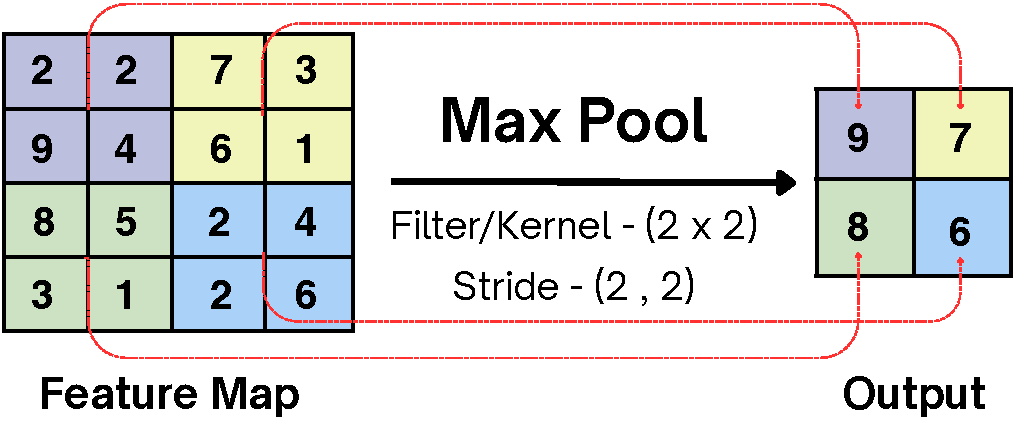
\includegraphics[width=0.75\textwidth]{max-pool.pdf}
  \caption{Ilustrasi proses max pooling pada feature map}
  \label{fig:max-pool}
\end{figure}

Pooling biasanya disebut sebagai detektor fitur.

\section*{STEP 4: Flatten}
\addcontentsline{toc}{section}{STEP 4: Flatten}
Flatten merupakan proses untuk mengubah data yang memiliki dimensi besar direduksi. Misal, jika memiliki data dengan 2 dimensi, maka setelah proses flattening, data tersebut akan menjadi 1 dimensi. Proses flattening ini dilakukan agar data dapat diteruskan ke fully connected layer.

\begin{figure} [H]
  \centering
  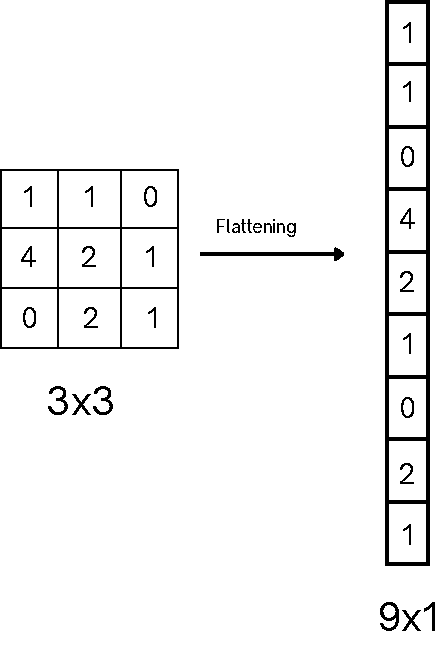
\includegraphics[width=0.3\textwidth]{flattening.pdf}
  \caption{Ilustrasi proses flatten}
  \label{fig:flatten}
\end{figure}

\section*{STEP 5: Fully Connected}
\addcontentsline{toc}{section}{STEP 5: Fully Connected}
\indent Fully connected atau dense layer merupakan kumpulan neuron yang saling terhubung dengan semua neuron pada layer sebelumnya. Satu neuron biasanya kita sebut sebagai perceptron. Perceptron ini memiliki bobot dan bias. Untuk ilustrasi perceptron bisa dilihat pada gambar dibawah ini.
\begin{figure} [H]
  \centering
  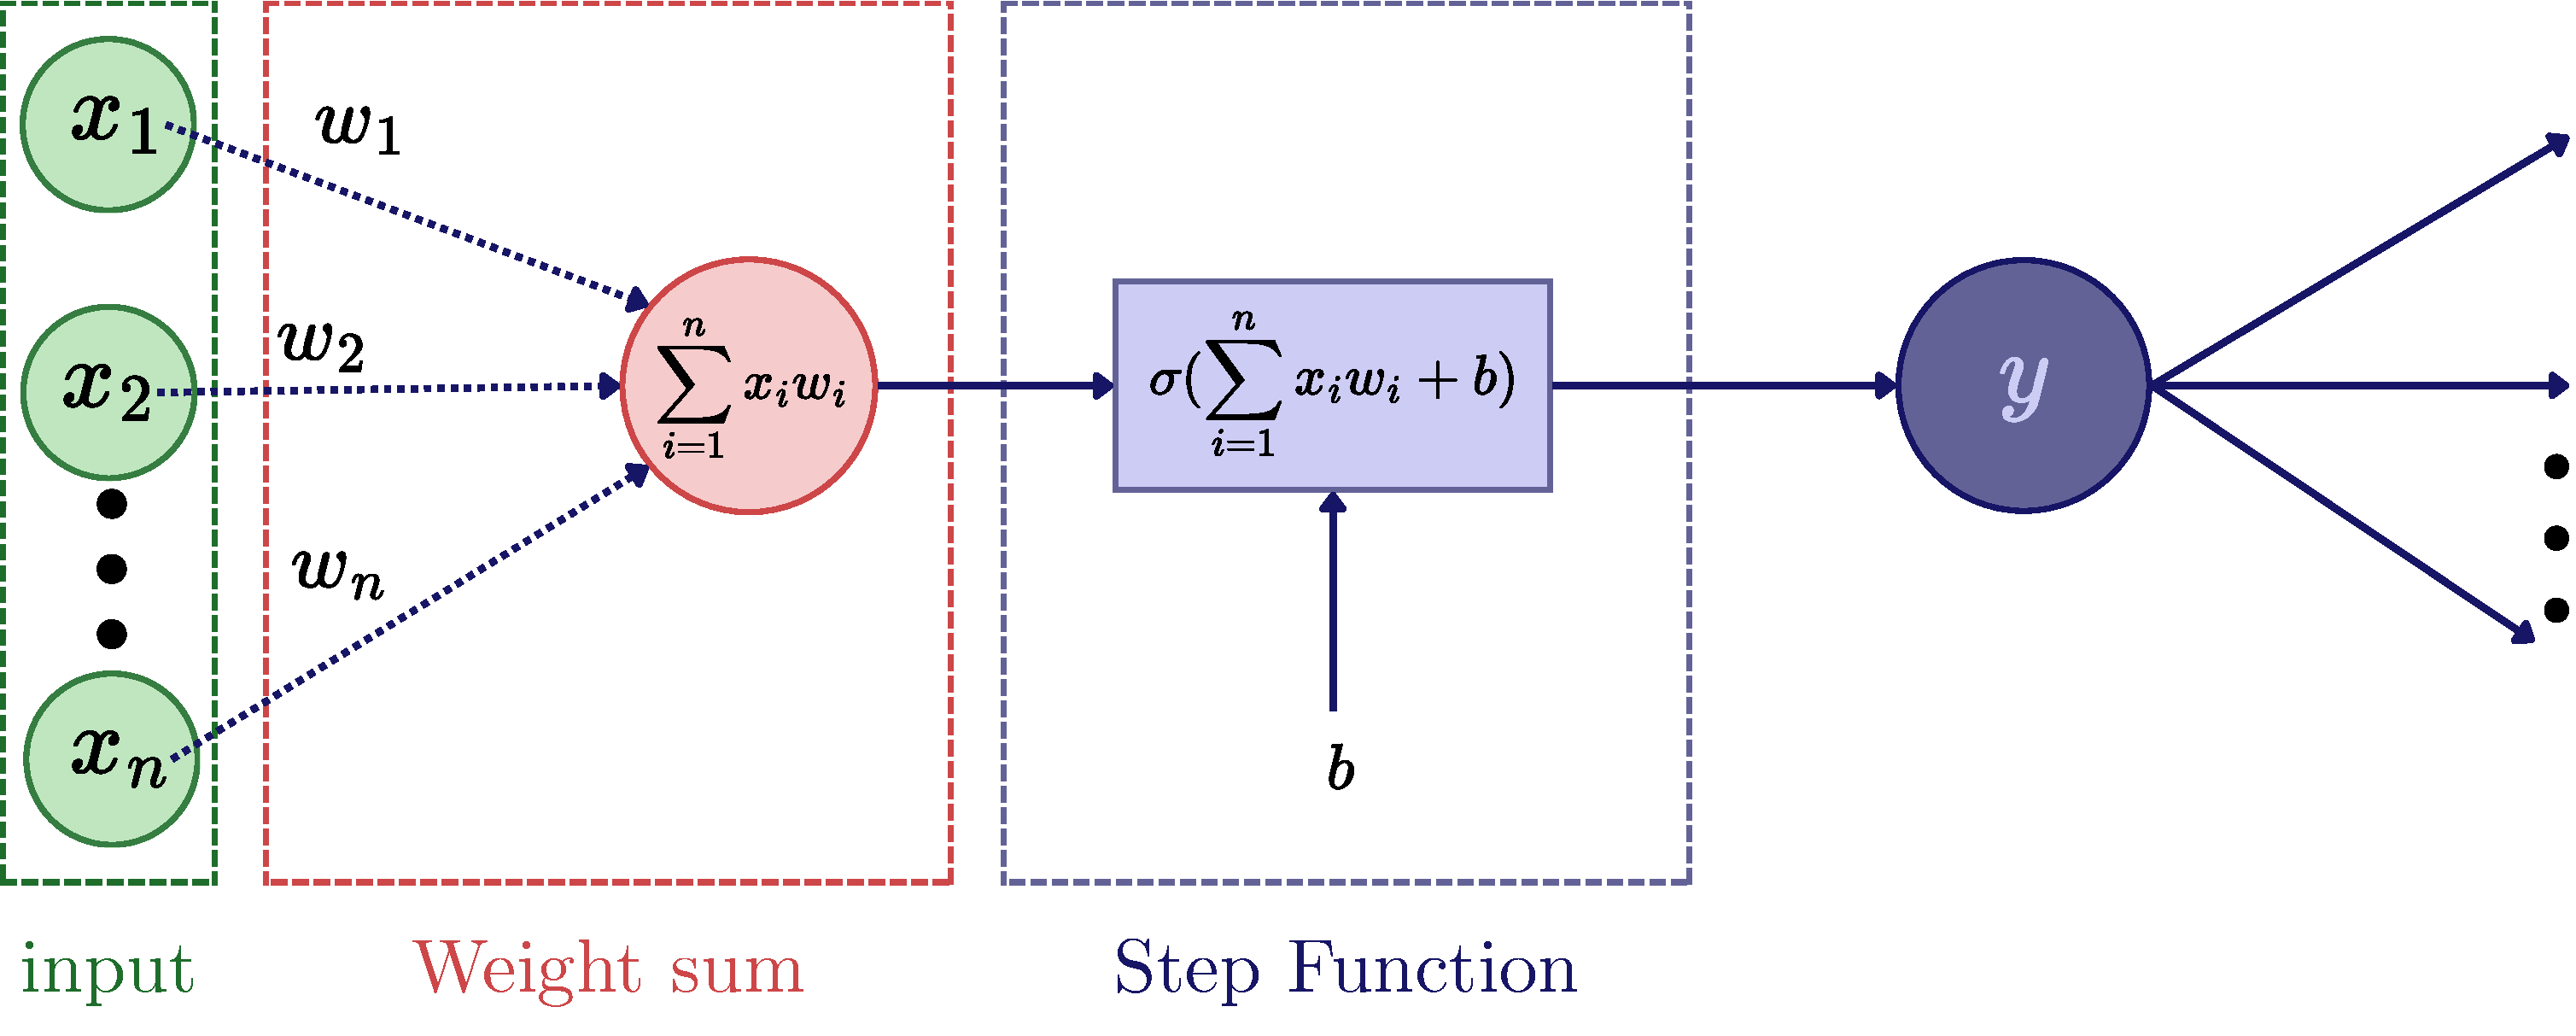
\includegraphics[width=0.8\textwidth]{perceptron.pdf}
  \caption{Ilustrasi perceptron}
  \label{fig:perceptron}
\end{figure}
Dari proses perceptron ini, apabila kita memiliki banyak neuron, maka kita bisa menyebutnya sebagai fully connected layer. Secara rumus matematis, bisa ditulis sebagai:
\begin{equation}
A^{(l)} = \sigma^{(l)}(W^{(l)}A^{(l-1)}+b^{(l)}), l = 1,2,\dots,L \label{eq:nnfeedforward}
\end{equation}
dengan $A^{(0)} = X$ sebagai input, $W^{(l)}$ adalah matriks bobot pada lapisan ke-$l$, $b^{(l)}$ adalah vektor bias pada lapisan ke-$l$, $\sigma^{(l)}$ adalah fungsi aktivasi non-linear pada lapisan ke-$l$, dan $L$ adalah jumlah total lapisan dalam jaringan.

\begin{figure} [H]
  \centering
  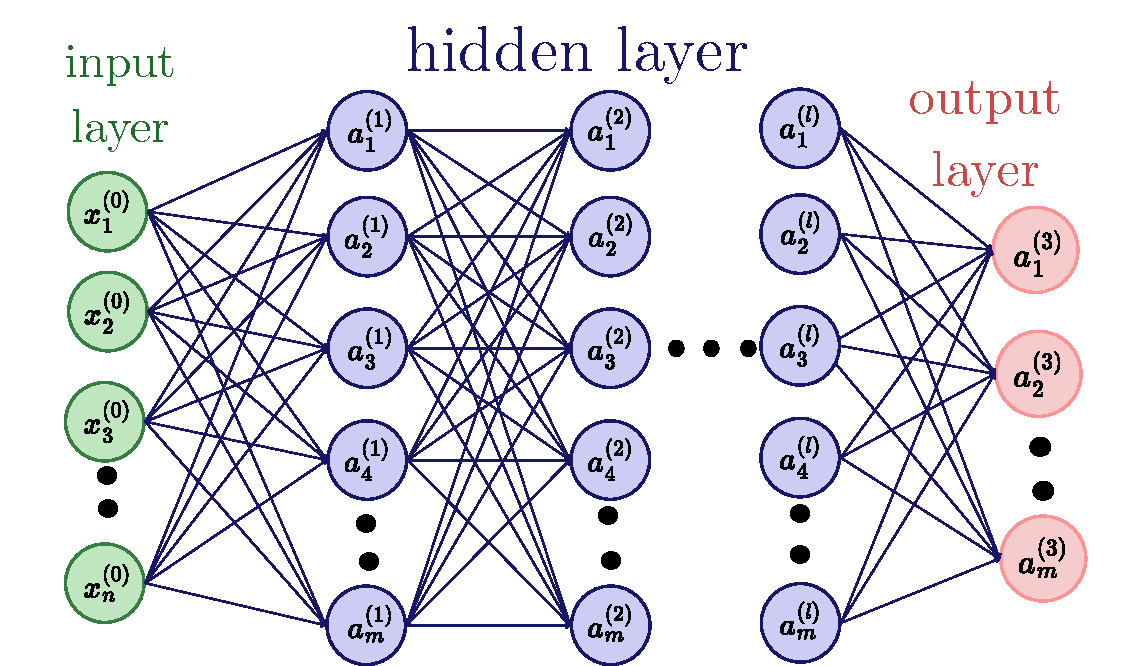
\includegraphics[width=0.8\textwidth]{nn-arsitektur.pdf}
  \caption{Ilustrasi arsitektur neural network dengan beberapa lapisan fully connected}
  \label{fig:nn-arsitektur}
\end{figure}

\section*{STEP 6: Softmax}
\addcontentsline{toc}{section}{STEP 6: Softmax}
Softmax merupakan fungsi aktivasi yang mengubah ke distribusi probabilitas. Maksudnya adalah output dari softmax akan memiliki nilai antara 0 dan 1, dan jumlah dari semua output softmax adalah 1. Rumus dari softmax adalah:
\begin{equation}
  \sigma(z_i) = \frac{e^{z_i}}{\sum_{j=1}^{n} e^{z_j}}
\end{equation}
Pada projek ini, softmax digunakan pada output layer fully connected layer, karena cocok digunakan untuk klasifikasi. Softmax ini akan mengubah model yang hasilnya masih raw menjadi probabilitas, sehingga dapat digunakan untuk menentukan kelas dari input data. Softmax ini seperti cross-entropy loss (kita bahas di step selanjutnya).

\section*{STEP 7: Loss Function}
\addcontentsline{toc}{section}{STEP 7: Loss Function}
Loss function merupakan fungsi yang digunakan untuk mengukur seberapa baik model dalam memprediksi output. Pada projek ini, loss function yang digunakan adalah cross-entropy loss, karena cocok digunakan untuk klasifikasi. Untuk rumus cross-entropy yang digunakan pada projek ini adalah versi binary, yaitu:
\begin{equation}
  BCE = -\frac{1}{N} \sum_{i=1}^{N} [y_i \cdot \log(p_{i}) + (1 - y_i) \cdot \log(1 - p_{i})]
\end{equation}
yang dimana:
\begin{itemize}
  \item $N$ adalah jumlah sampel
  \item $y_i$ adalah true label dari sampel ke-$i$ (0 atau 1)
  \item $p_i$ adalah model-predicted probabilitas untuk class 1 untuk sampel i
\end{itemize}

\section*{STEP 8: Backpropagation}
\addcontentsline{toc}{section}{STEP 8: Backpropagation}
% Fully connected bisa kita sebut sebagai forward-pass, mengapa demikian?karena di fully connected tidak melakukan secara optimasi. Oleh karena itu, dilakukan optimasi yang kita namakan sebagai Backpropagation.

\section*{STEP 9: Gradient Descent}
\addcontentsline{toc}{section}{STEP 9: Gradien Descent}
\section*{STEP 10: Evaluasi Model}
\addcontentsline{toc}{section}{STEP 10 : Evaluasi Model}
(bikin epoch, batch size, dan learning rate sebagai hyperparameter, dan buat grafik loss function dan akurasi). Seberapa pengaruhnya dan tam
\section*{Kesimpulan}


% ============================================================
\begin{thebibliography}{99}
% ============================================================

\bibitem{goodfellow2016deep}
Goodfellow, I., Bengio, Y., \& Courville, A. (2016). \textit{Deep Learning}. MIT Press.
\href{https://www.deeplearningbook.org/}
{link}.

\bibitem{ChittaRanjan2020}
Chitta Ranjan, S., \& Saha, S. (2020). \textit{Understanding Deep Learning Application in Rare Event Prediction}. Springer.
\end{thebibliography}

\end{document}

%keep resource:
%https://medium.com/@onally.sourour9/max-pooling-in-cnns-why-it-matters-and-how-it-works-60c590bca8b9

%https://www.geeksforgeeks.org/deep-learning/introduction-to-pooling-layer-cnn/

%https://medium.com/@muhammadshoaibali/flattening-cnn-layers-for-neural-network-694a232eda6a

% https://fdsmlhn.github.io/2017/11/02/Understanding%20im2col%20implementation%20in%20Python(numpy%20fancy%20indexing)/

%https://www.geeksforgeeks.org/machine-learning/what-is-cross-entropy-loss-function/
